\documentclass[12pt]{article}

% MATH397MP-benjaminnewman.pdf
% use subject header MATH397MP

\usepackage{epsfig}
\usepackage{graphicx}
\usepackage{fancyvrb}
\usepackage{enumitem}
\usepackage{amsmath}
\usepackage{hyperref}
\usepackage{animate}


\usepackage{Bridges_LaTeX_Style}

\setlist{nosep}

\title{3D Rendering in Postscript}
\author{Ben Newman}
\begin{document}
	\maketitle
	\newpage
	\section{Overview}
	For my midterm project, I created a 3d rendering library in only Postscript, as well as some cool 3d renders (using the library). It still needs a lot of work, but it is certainly capable of creating simple renders with simple objects as well as slightly more sophisticated animations using Ghostscript. I started this library out with isometric rendering, and then moved on to perspective rendering, which is where I still am. This project has helped me understand 3d rendering much better, and I hope to continue this project at least through the semester, if not further. It also helped me remember and learn more about linear algebra, even requiring me to implement my own matrix multiplication in Postscript.
	\section{Isometric Projection}
	The first rendering method I implemented was Isometric Projection. This method is mainly used in technical drawings, as it makes angles much easier to draw for the most part, simplifying the process.
	The method to obtain the proper projection coordinates with Isometric projection is relatively simple, requiring only two matrix multiplications (where one of the matrices is the 3d coordinates, one doesn't change, and the last is based off of the camera angle). The equation I used was: 
	\begin{align*}
		&a_x=B_{11},a_y=B_{21}\\
		&\text{Where: }\\&\alpha=\arcsin{\left(\tan{30^\circ}\right)}\text{ (Rotation around the horizontal axis)}\\
		&\beta=45^\circ\hspace{61pt}\text{ (Rotation around the vertical axis)}\\
		&c \text{ is the 3d coordinates}\\
		&B=\left[ {\begin{array}{ccc}
				1 & 0 & 0 \\
				0 & \cos\alpha & \sin\alpha \\
				0 & -\sin\alpha & -\cos\alpha \\
		\end{array} } \right]
		\cdot 
		\left[ {\begin{array}{ccc}
				\cos\beta & 0 & -\sin\beta \\
				0 & 1 & 0 \\
				\sin\beta & 0 & \cos\beta \\
		\end{array} } \right]
		\cdot
		\left[ {\begin{array}{c}
			c_x \\ c_y \\c_z
		\end{array} } \right]
	\end{align*}
	This calculation is relatively light, and for most cases can be run in real time with a few objects. Here's a simple example of a cube rendered in isometric -- note that it's not really clear which way the cube is facing. The reason that there are triangles, and not just "squares" is because I've chosen to split up every square face into two triangles to be rendered.\\
	\begin{align*}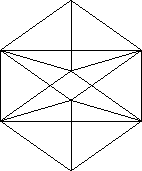
\includegraphics[height=100pt]{animations/isocube.png}\end{align*}\\
	 However, because of the way that the points are projected, objects don't scale based off of the camera -- In fact, there is no defined camera location. This limitation prompted me to instead look to Perspective Projection.
	\section{Perspective Projection}
	The second method that I implemented was Perspective Projection. This method is the main method used in most modern 3d games. It is certainly a little heavier time-complexity wise, requiring more matrix multiplications, but looks a lot better and handles distance much better than isometric projection. The equation I used (adapted from Dhirgham Murran's equations) was:\\
	\begin{align*}
		&b_x=\frac{e_z}{d_z}\cdot d_x+e_x\\
		&b_y=\frac{e_z}{d_z}\cdot d_y+e_y\\
		&\text{Where}\\
		&\begin{bmatrix}d_x\\d_y\\d_z\end{bmatrix}=\begin{bmatrix}1&0&0\\0&\cos\theta_x&\sin\theta_x\\0&-\sin\theta_x&\cos\theta_x\end{bmatrix}
		\cdot
		\begin{bmatrix}\cos\theta_y&0&-\sin\theta_y\\0&1&0\\\sin\theta_y&0&\cos\theta_y\end{bmatrix}
		\\&\cdot
		\begin{bmatrix}\cos\theta_z&\sin\theta_z&0\\-\sin\theta_z&\cos\theta_z&0\\0&0&1\end{bmatrix}
		\cdot\left(\begin{bmatrix}p_x\\p_y\\p_z\end{bmatrix}-\begin{bmatrix}c_x\\c_y\\c_z\end{bmatrix}\right),\\
		&\theta\text{ is the Euler angles of the camera,}\\
		&p\text{ is the point in 3d space,}\\
		&\text{and }c\text{ is the camera's location in 3d space.}
		\\
	\end{align*}
	This perspective rendering allowed me to rotate and move the camera around, which let me create renders like this (the animation will only play in a javascript-enabled pdf viewer):\\
	\begin{align*}\animategraphics[loop,controls,width=100pt]{15}{animations/GOL/frame-}{0}{1}\end{align*}\\
	With the previous isometric technique, this sort of rotation would not have been feasible, or looked nearly as normal.
	\section{Drawbacks}
	With the current version of the code, there is no proper support for any form of culling (i.e. removing faces behind other faces, or faces that aren't within the viewport). And, unfortunately, due to that, I also cannot realistically implement any sort of lighting, shading, or non-uniform solid coloring because the faces on the back of objects will show through in front of the front faces, which causes renders to not make sense or look impossible. The culling will also significantly speed up the rendering process, as in many cases around half of the faces that are being rendered do not have to be rendered at all.\\The one bug I am aware of in my library code is the fact that all of the Z values have to be scaled down by 0.0016 -- I'm sure there's a simple fix/reason, but I haven't been able to find it yet. It's not too big of an issue, but does cause bugs frequently.\\Another frequent bug I encounter is when objects are drawn very close to the camera -- they aren't clipped, so they sometimes render over the camera in very wild lines that extend across the screen.
	\section{Next Steps}
	I plan to continue to develop this 3d renderer as long as I can -- I certainly hope to at least overcome the obstacles outlined in the drawbacks section. What I'm currently working on is a proper depth buffer, which is the first step to being able to have culling (at least depth based culling). Once that's been completed, the next step is to implement some simple form of lighting, to be able to differentiate between faces without having to render the edges between them. This will open up many opportunities for much more interesting renders, although it will significantly decrease performance. 
	\section{Code and examples}
	The following link is the main file of the 3d rendering (i.e. the "library"):
	\href{https://gist.github.com/bn0367/3b670a37fc172aa1ae74cbbafd8cbb5a}{3d.eps}\\
	A few cool examples: 
	\begin{align*}\animategraphics[loop,controls,width=250pt]{30}{animations/icosphere_sin/frame-}{0}{1}\end{align*}\\
	\begin{align*}\animategraphics[loop,controls,width=250pt]{30}{animations/icospheres/frame-}{0}{1}\end{align*}\\
\end{document}